\documentclass[tikz, border=5pt]{standalone}
\usetikzlibrary{calc,angles,quotes}
\tikzset{
  > = {stealth},
  inertial frame/.style = {x={(-160:1.5cm)}, y={(-20:1.5cm)}, z={(90:2.5cm)}},
}

\begin{document}
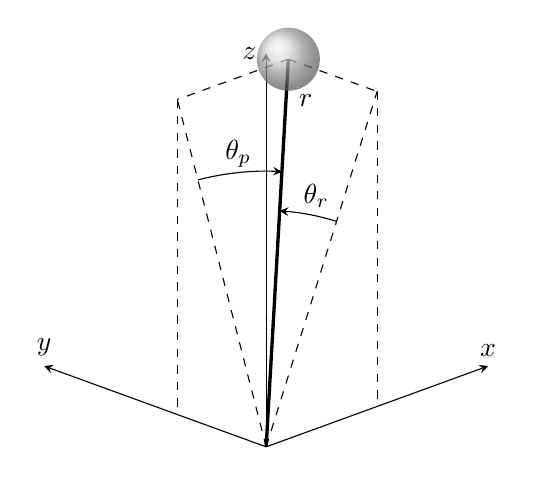
\begin{tikzpicture}[scale=2, inertial frame]

  %% define coordinates 
  \coordinate (origin) at (0,0,0);
  \coordinate (CoM) at (-0.5,-0.4,0.8);
  \coordinate (CoM_x) at (-0.5,0,0.8);
  \coordinate (CoM_x0) at (-0.5,0,0);
  \coordinate (CoM_y) at (0,-0.4,0.8);
  \coordinate (CoM_y0) at (0,-0.4,0);
  
  % draw inertial frame
  \draw[->] (origin) -- (-1,0,0) node[above] {$x$};
  \draw[->] (origin) -- (0,-1,0) node[above] {$y$};
  \draw[->] (0,0,0) -- (0,0,1) node[left] {$z$};

  % draw inverted pendulum
  \draw[very thick] (origin) -- (CoM) node[below=15, right] {$r$};

  % draw x projection of the inverted pendulum
  \draw[dashed] (CoM) -- (CoM_x);
  \draw[dashed] (CoM_x) -- (CoM_x0);
  \draw[dashed] (origin) -- (CoM_x);

  % draw y projection of the inverted pendulum
  \draw[dashed] (CoM) -- (CoM_y);
  \draw[dashed] (CoM_y) -- (CoM_y0);
  \draw[dashed] (origin) -- (CoM_y);

  % draw theta_r angle
  \pic [draw, ->, angle eccentricity=0, angle radius = 3cm] {angle = CoM_x--origin--CoM};
  \node[left=22, below = 30] at (CoM_x) {$\theta_r$};

  % draw theta_p angle
  \pic [draw, <-, angle eccentricity=0, angle radius = 3.5cm] {angle = CoM--origin--CoM_y};
  \node[right=22, below = 11] at (CoM_y) {$\theta_p$};

  % fraw the CoM of the robot  
  \shade[ball color = gray!40, opacity = 0.7] (CoM) circle (0.20cm);
\end{tikzpicture}
\end{document}
